\documentclass[11pt]{article}
\usepackage{graphicx}
\usepackage{url}
\usepackage{epigraph}
\usepackage{float}
\usepackage{wrapfig}
\usepackage{listings}
\usepackage{multirow}
\usepackage{hyperref}
\usepackage{amsfonts}
\usepackage{amsmath}
\usepackage{array}
\usepackage{etoolbox}
\usepackage{yax}



\title{\rmfamily\normalfont{Nexus Proof-of-Stake with Tritium Trust}}

\author{Colin Cantrell\\
\and Scott Simon}

\date{September 28, 2019}
    
\begin{document}
\pagenumbering{gobble}

\begin{figure}
    \centering
	
\includegraphics[width=0.44\textwidth]{images/logo.png}
\end{figure}

\maketitle

\newpage
\pagenumbering{arabic}

\bigskip

\section{Introduction}
The Nexus network operates using three channels for producing valid blocks and minting new NXS currency -- two Proof-of-Work channels and one Proof-of-Stake channel. The original Proof-of-Stake channel introduced the concept of trust as a core component to measure consistent and honest contribution by a node to the Nexus network. With the release of Tritium Trust, this trust system is revised and enhanced. Through it, Nexus has improved its Proof-of-Stake channel for future growth and laid the groundwork for development of a Trust and Reputation system as well as Trust Locks in future releases of the TAO framework.\footnote{see "The Nexus Three Dimensional Chain Simplified" by gjsteele71\\ \url{https://steemit.com/bitcoin/@gjsteele71/the-nexus-three-dimensional-chain-simplified}} \\ 

\noindent This paper discusses the updates in the Tritium Trust release with respect to how they affect Nexus Proof-of-Stake.

\bigskip

\section{Proof-of-Stake}

\subsection{What is Proof-of-Stake?}
The concept of Proof-of-Stake was first introduced in 2012 by King \& Nadal\footnote{King, S.; Nadal, S. (August 12, 2012). ”PPCoin: Peer-to-peer crypto-currency  with  proof-of-stake” \url{https://peercoin.net/assets/paper/peercoin-paper.pdf}} as a proposal to develop a form of mining that addressed the growing issue of energy consumption related to Bitcoin Proof-of-Work mining. It developed the idea of using proof of ownership of a currency as a means for granting the ability to mine blocks on the blockchain. These blocks would include a \textit{coinstake} transaction that rewarded the currency owner in a manner similar to how coinbase transactions reward Proof-of-Work miners.\\

\noindent Early incarnations of Proof-of-Stake built around the idea of \textit{coin age}, defined as a measure of the holding period for the currency. Upon reaching a specified coin age, the currency owner would gain the ability to stake a new block on the blockchain.\\

\noindent This design was elegant in how it solved the issue of energy efficiency, while having the drawback that the currency owner didn't have to do anything. They could simply leave their wallet off, only activating it upon reaching the age level needed to generate blocks and earn rewards.\\

\noindent As a result, Proof-of-Stake was gradually refined. It remained a form of energy efficient mining, but evolved into a mechanism whereby currency holders can earn rewards proportional to the size of their holdings by keeping a node up and running at all (or nearly all) times, thus contributing to the operation and security of the blockchain network.\\

\subsubsection{Staking Concepts}

\paragraph{Time} ~\\
Proof-of-stake introduced the use of time as an input to mining, initially through the use of coin age. Using time in this manner inhibits the application of raw computational power to solve blocks more quickly, thus promoting energy efficiency. Requiring a significant time investment also introduces an external cost to staking that improves network security. 

\paragraph{Weight} ~\\
Different Proof-of-Stake systems use varying ideas for the concept of weight. Basically, all of these introduce an approach where the ability of currency owners is weighted in such a manner that some have a higher chance to generate blocks than others. Coin age based systems often weighted based on number of coins owned, so if two people had the same holding period, but one had twice as many coins as the other, that one would have twice as much opportunity to generate staking blocks.

\paragraph{Minting Rate} ~\\
This rate, expressed as a percentage, is used to calculate the size of the coinstake reward in a Proof-of-Stake block. Over time, it has become commonly referred to as interest rate because it operates in a similar manner and people already have an understanding of that term. But anyone staking should understand that their coins are not actually earning interest. They are earning staking rewards in return for helping operate and secure the blockchain network.\\

\noindent Defining the minting rate is an important aspect of a staking system. Too low and rewards are not significant enough to encourage nodes to stake. Too high and the resulting inflation of the currency supply will erode its value, especially when compounded over time.

\paragraph{Distribution Problem} ~\\
A pure Proof-of-Stake based currency suffers from a chicken-and-egg problem that you cannot create staking blocks unless you first have coins to stake. Therefore, most currencies that use Proof-of-Stake also employ an initial distribution based on Proof-of-Work mining, at least temporarily.\\

\noindent Nexus has realized the value of this type of multi-channel system as it relates to network security, and uses 3 minting channels, two based on Proof-of-Work and one based on Proof-of-Stake. This system also supports initial distribution via the Proof-of-Work channels.

\paragraph{Nothing At Stake Problem} ~\\
Proof-of-work mining requires the consumption of large amounts of energy, which is a valuable resource. A basic Proof-of-Stake system, on the other hand, only uses resources already within the network, and you don’t lose anything for behaving dishonestly or signing all blocks on any fork in the chain, then attempting to build on all forks. There is no cost or “nothing at stake” for doing so. It is a hypothetical problem that nevertheless must be addressed by any staking system.\\

\noindent In addition to other benefits, the use of multiple channels in Nexus also addresses this problem, as the disparate channels keep each other honest. The Nexus network also employs checkpoints that protect against attacks, and introduces the concept of trust (see below) to create a cost to misbehavior. 

\paragraph{51\% Attack} ~\\
As with other forms of mining, Proof-of-Stake systems can potentially be exposed to a 51\% attack that gives the attacker control of the network. Under this type of system, however, it requires an attacker to gain control of 51\% of the currency on the network. This becomes incredibly expensive to do, and thus highly unlikely, especially when a staking system combines it with a significant time requirement for generating staking weight.\\

\noindent Within Nexus, not only is it highly unlikely a 51\% attack could occur on the Proof-of-Stake channel, but an attacker would also have to gain control of both Proof-of-Work channels to be successful. \\

\bigskip

\section{Nexus Proof-of-Stake}
The Tritium Trust release builds on the previous Nexus Proof-of-Stake system. It employs many of the staking concepts developed in previous staking systems, enhances them, and adds new concepts that further enhance performance and security for Proof-of-Stake.\\

\subsection{Genesis}
Before a new wallet can stake successfully on the Nexus network, it must first create a trust key. This key is created by successfully mining its first 
Proof-of-Stake block, a process referred to as Genesis. The initial coinstake transaction is thus the Genesis transaction. \\

\begin{wrapfigure}{r}{0.63\textwidth}
    \centering
    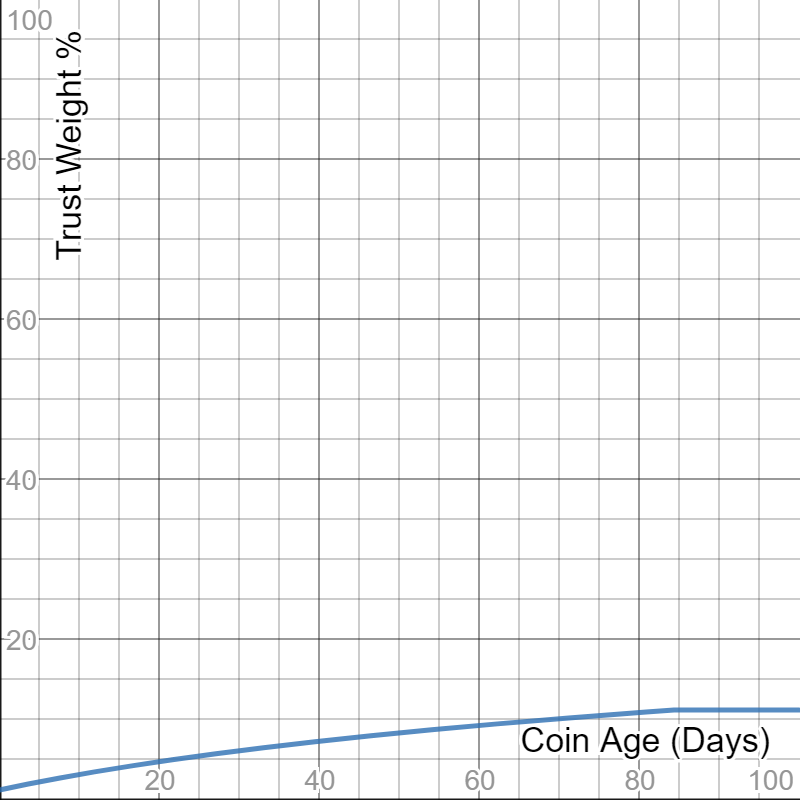
\includegraphics[width=0.55\textwidth]{images/preGenesisTrustWeight.png}
    \caption{Trust Weight pre-Genesis \label{fig:preGenesisTrust}}
\end{wrapfigure}

\noindent While staking for Genesis, the node will gradually build Trust Weight. Over time, this increases the chances of successfully generating a Genesis transaction. The pre-Genesis value for trust only applies to the Genesis process and is based on coin age. It caps at a level of 11\% of maximum, as shown in Figure \ref{fig:preGenesisTrust}.\\

\noindent When the Genesis transaction is created, the wallet also creates the trust key and transfers all balance to that key for staking. This has no impact on the wallet balance, besides moving it to the new key.\\

\subsection{Trust}
Upon creating a new trust key, the network immediately begins to build trust on that key. Continued staking will generate additional Trust transactions whenever the node successfully mines a Proof-of-Stake block. Each of these rewards the wallet owner for continuing to operate their node.\\

\noindent As with the Genesis transaction, Trust transactions will also transfer any new NXS sent to the wallet onto the trust key for staking. \\

\begin{wrapfigure}{r}{0.63\textwidth}
    \centering
    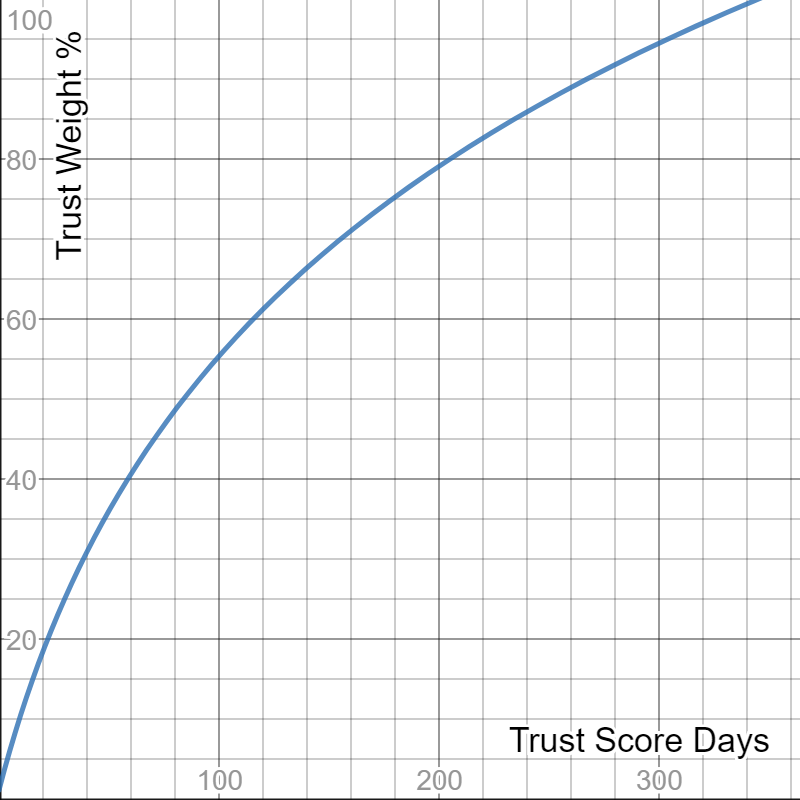
\includegraphics[width=0.55\textwidth]{images/trustWeight.png}
    \caption{Trust Weight \label{fig:trustWeight}}
\end{wrapfigure}

\noindent Trust is measured by the key’s trust score, which initially equals the age of the trust key. As long as the key does not undergo decay (see section 3.5) or get penalized for misbehavior, trust score will continue to grow in this manner.\\

\noindent The trust score reflects the network’s level of trust in the node as a measure of the time it has been operating and producing new blocks in an honest and trustworthy manner. The significant investment in time needed to build trust score enhances the security of the overall network.\\

\noindent The trust score is used to calculate Trust Weight. Increased Trust Weight improves the chances of successfully staking a new block.\\

\noindent Figure \ref{fig:trustWeight} depicts how Trust Weight, expressed as a percentage of maximum value, grows as trust score, expressed as days of time, increases.\\

\subsection{Interest Rate}
The size of the staking reward is based on the current interest rate (minting rate) for the wallet’s trust key. The Genesis process uses a base rate of 0.5\% (annual). After Genesis, future Trust transactions use an interest rate derived from the trust score.\\

\noindent This interest rate will range from the base rate of 0.5\% up to a maximum of 3.0\% after the trust key has accrued one year worth of aggregate trust score. \\

\begin{figure}[h!]
    \centering
    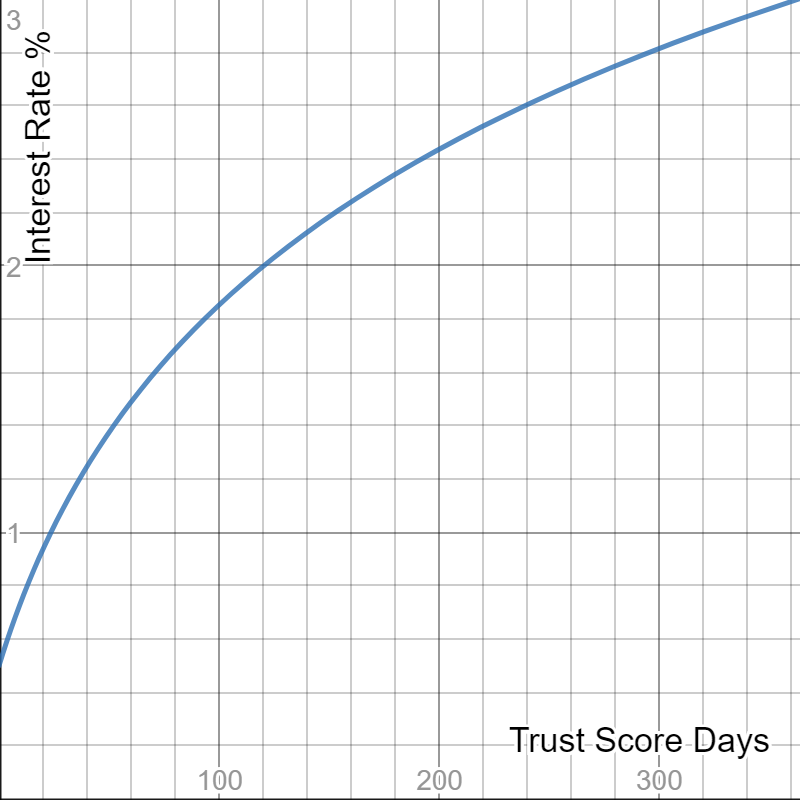
\includegraphics[width=0.55\textwidth]{images/interestRate.png}
    \caption{Interest Rate \label{fig:interestRate}}
\end{figure}

\noindent Figure \ref{fig:interestRate} depicts how Interest Rate, expressed as an annual percentage, grows as trust score, expressed in days of time, increases. Interest Rate caps when it reaches the maximum value of 3\%.\\

\subsection{Block Weight}
To continue accruing trust score, a wallet must successfully generate a new Trust transaction within a three day time requirement. The use of Block Weight serves two functions in this respect.\\

\noindent First, it acts as a timer. When Block Weight reaches 100\%, the trust key will begin to undergo decay (see section 3.5).\\

\noindent Second, a higher value for Block Weight increases the chances of successfully staking a block. Thus, as it gets closer to the 3-day time limit, chances to generate the required Trust transaction increase.\\

\begin{figure}[h!]
    \centering
    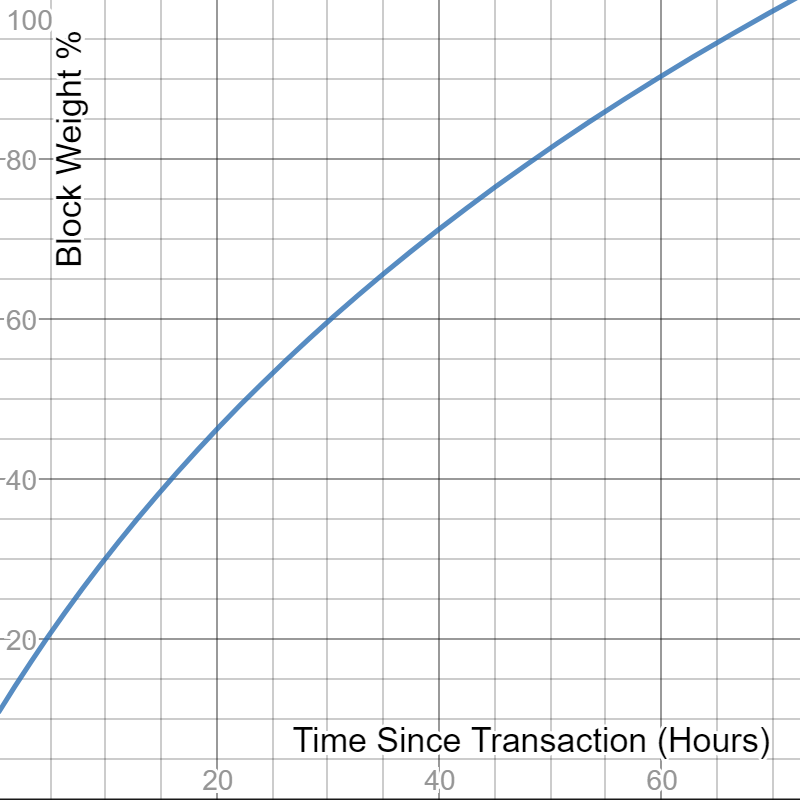
\includegraphics[width=0.55\textwidth]{images/blockWeight.png}
    \caption{Block Weight \label{fig:blockWeight}}
\end{figure}

\noindent Figure \ref{fig:blockWeight} depicts how Block Weight, expressed as a percentage of maximum value, grows over three days of time.\\

\subsection{Decay}
Tritium Trust introduces the process of Decay if staking fails to generate a Trust transaction within the required time limit. The trust key does not expire. Instead, it will reset back to the level of its previous Trust transaction, and begin to decay from that point. Trust score decays at a 3:1 ratio to the rate it was earned.\\
\begin{equation}
\resizebox{.50\hsize}{!}{$T_s = T_p - 3 \cdot (B_t - 259200)$}
\end{equation}

\noindent Where $T_s$ = new trust score, $T_p$ = prior trust score at last transaction, $B_t$ = time since last stake block, and 259200 is three days expressed in seconds.\\

\noindent Normally, Trust Weight depicted in Figure \ref{fig:trustWeight} moves forward along the curve as trust score grows. During decay, you can think about it as moving backwards along the same curve. The same would be true of Interest Rate in Figure \ref{fig:interestRate}. \\

\noindent If, at any time, the wallet finds a new stake block and generates a Trust transaction, Block Weight is reset, Decay ends, and trust score begins accruing again from that point. \\

\noindent The benefit of Decay in Tritium Trust is that trust keys no longer expire. They simply add or subtract trust score. Those who have invested a lot of time staking a trust key won’t have that key expire as the result of a random event such as a power outage. Trust might decay somewhat, but that can be earned back.\\

\noindent The time investment that it takes to build trust score, combined with this introduction of the ability to both add and subtract trust score, also supports administration of trust penalties for misbehavior or dishonesty, and forms the basis for future application as part of a Trust and Reputation system within the Nexus TAO framework.\\

\bigskip

\section{Beginning Staking with a New Wallet}

\subsection{Establishing a Trust Key}
Trust is not something that is easily earned in real life. Nor is it easily established in Nexus Proof-of-Stake. Establishing a new trust key is a process. This process can take some time, especially for those staking with smaller balances.\\

\noindent After Genesis, Trust Weight is low so transactions are less frequent. It is normal that a new key might not earn a Trust transaction within the required 3-day period. The key is also new, so Decay will immediately reduce trust score and interest rate back to starting values (the trust level of its prior transaction) as soon as Block Weight reaches 100\%.\\ 

\noindent From that point, Block Weight will stay at 100\%, while Trust Weight and Interest Rate stay at minimum starting values (1.11\% and 0.5\% respectively). These value will not change until it finds a staking block and generates a Trust transaction. Then, Trust Weight and Interest Rate begin to grow again.\\

\noindent This cycle may repeat multiple times before a new key can generate enough Trust transactions to successfully establish itself and continue growing. This is normal. It is all part of earning trust.\\

\subsection{Nexus Staking Requirements}

\paragraph{Minimum Balance} ~\\
There is no minimum balance for staking with Tritium Trust on the Nexus network. The general guideline is to have at least 1000 NXS to successfully establish a new trust key and have it grow. But that is just a guideline. It may take awhile, but a smaller balance could possibly establish a key successfully. Even if it doesn’t, it will still generate occasional Trust transactions that earn staking rewards at the starting Interest Rate.

\paragraph{Minimum Coin Age} ~\\
The Genesis process requires a minimum coin age of 72 hours before allowing the wallet to stake. A new wallet that just received its first NXS must wait this long to begin staking. Any sending or receiving of balance affects coin age, also, which may impact the ability to start staking. 

\paragraph{Maturity} ~\\
Staking is a form of mining, and, as with Proof-of-Work, must wait a minimum period for a staking transaction to mature. For Nexus, maturity takes 120 blocks (about 90 minutes). During this time, the wallet balance will not be available for other use. 

\bigskip

\section{Technicals}
This section revises and replaces the technical details originally published in the Nexus white paper. \footnote{Nexus: A Peer-to-Peer Network \url{https://nexusearth.com/nexus-white-paper/}}

\subsection{Trust Weight}
\noindent Nexus Proof-of-Stake uses two distinct calculations to determine current Trust Weight, one based on coin age during the Genesis process and one based on current trust score for the remainder of staking.\\

\noindent The numeric value of Trust Weight ranges from 1 to 90, although it is commonly expressed as a percentage of its maximum value.\\

\paragraph{Pre-Genesis Trust Weight} ~\\
\begin{equation}
\resizebox{.65\hsize}{!}{$W_{t} = Min(10.0, \frac{9.0 \cdot ln(\frac{2 \cdot a_c}{7257600} + 1)}{ln(3)} + 1.0)$}
\end{equation}

\noindent Where $a_c$ is the current coin age.\\

\paragraph{Staking Trust Weight} ~\\
\begin{equation}
\resizebox{.65\hsize}{!}{$W_{t} = Min(90.0, \frac{44.0 \cdot ln(\frac{2 \cdot T_{s}}{7257600} + 1)}{ln(3)} + 1.0)$}
\end{equation}

\noindent Where $T_{s}$ is the current trust score.\\


\subsection{Interest Rate}
\noindent For the Genesis transaction, the staking reward is calculated using the starting interest rate of 0.5\%. Trust transactions use the current interest rate calculated from accumulated trust score.\\
 
\begin{equation}
\resizebox{.65\hsize}{!}{$R_{m} = \frac{0.025 \cdot ln(\frac{9 \cdot T_{s}}{31449600} + 1)}{ln(10)} + 0.005$}
\end{equation}

\noindent Where $T_{s}$ is the current trust score and $R_{m}$ is the resulting minting rate (interest rate).\\


\subsection{Staking Rewards}
\paragraph{Genesis Transaction} ~\\
\begin{equation}
\resizebox{.50\hsize}{!}{$S_{r} = \frac{C_{w} \cdot 0.005 \cdot a_c}{31449600}$}
\end{equation}

\noindent Where $C_{w}$ is the current wallet balance and $S_{r}$ is the staking reward.

\paragraph{Trust Transaction} ~\\
The Trust reward has two possible components. The first part is the reward for balance staked on the trust key, based on the block time (time since last Trust transaction). The second part accounts for any new balance added to the wallet. This balance only earns rewards for the time since adding it.\\

\begin{equation}
\resizebox{.50\hsize}{!}{$S_{t} = \frac{C_{t} \cdot R_{m} \cdot B_{t}}{31449600}$}
\end{equation}

\noindent Where $C_{t}$ is the trust key balance, $B_{t}$ is the block time, and $S_{t}$ is the staking reward from the trust key.\\

\begin{equation}
\resizebox{.50\hsize}{!}{$S_{n} = \frac{C_{n} \cdot R_{m} \cdot a_c}{31449600}$}
\end{equation}

\noindent Where $C_{n}$ is any new balance added to the wallet, $a_c$ is the coin age of that new balance, and $S_{n}$ is the staking reward from any new balance. This balance is then transferred to the trust key for further staking.\\

\noindent The total reward for a trust transction $S_{r} = S_{t} + S_{n}$


\subsection{Block Weight}
The Genesis process does not use Block Weight and its value remains zero. After Genesis, the numeric value of Block Weight ranges from 1 to 10, although it is commonly expressed as a percentage of its maximum value.\\

\begin{equation}
\resizebox{.65\hsize}{!}{$W_{b} = Min(10.0, \frac{9.0 \cdot ln(\frac{2 \cdot B_{t}}{259200} + 1)}{ln(3)} + 1.0)$}
\end{equation}\\


\subsection{Stake Weight}
Stake Weight is a derivative measure that depicts the combined effect of Trust Weight and Block Weight on overall chances to generate a block. The Required Threshold (see Section 5.6) uses Trust Weight and Block Weight directly, so the value of Stake Weight is for informative purposes only.\\

\begin{equation}
\resizebox{.40\hsize}{!}{$W_{s} = W_{t} + W_{b}$}
\end{equation}

\noindent As shown previously, absolute values for Trust Weight range from 1-90 and Block Weight from 1-10. Thus, Stake Weight will range from 2-100, and can be directly expressed as a percentage.\\


\subsection{Required Threshold}

\begin{equation}
\resizebox{.5\hsize}{!}{$R_{t} = \frac{(108 - W_{t} - W_{b}) \cdot 1000}{(C_{w} + S_{r})}$}
\end{equation}


\noindent The value for Energy Efficiency Threshold must be above this value for the wallet to attempt stake block generation.\\


\subsection{Energy Efficiency Threshold}

\begin{equation}
\resizebox{.22\hsize}{!}{$E_{t} = \frac{100 \cdot T_{b}}{N_{once}}$}
\end{equation}

\noindent Where $T_{b}$ is the time since the last block was added to the blockchain, in seconds.\\

\noindent The Nexus stake minter will iterate over the process of attempting to find a block hash that meets staking difficulty requirements, incrementing $N_{once}$ with each iteration. Whenever this causes the value for the Energy Efficiency Threshold to fall below the Required Threshold, it will stop.\\

\noindent As the time since the last block increases, so will the Energy Efficiency Threshold and it can begin iterating again. Higher Trust Weight, Block Weight, and balance allow for a greater number of iterations, increasing the possibility of finding a block.\\

\noindent This continues until it either finds a stake block or a new block is received from the network. Whenever a new block is received, the process resets and starts over.\\

\noindent This produces a non-intensive, efficient process whereby it attempts to generate new staking blocks using the parameters of the wallet’s trust key.\\




\end{document}
